\documentclass{beamer}
\usepackage[utf8]{inputenc}
\usepackage[frenchb]{babel}
\usepackage[T1]{fontenc}
\usepackage{graphics}
\usepackage{framed}
\usepackage{graphicx}
\usepackage{subcaption}
\usepackage{grffile}
\usepackage{longtable}
\usepackage{wrapfig}
\usepackage{rotating}
\usepackage[normalem]{ulem}
\usepackage{amsmath}
\usepackage{textcomp}
\usepackage{amssymb}
\usepackage{capt-of}
\usetheme{Madrid}

\title[Support pour Verificarlo]{Support de MPI et de la vectorisation dans Verificarlo}
\subtitle{Master Calcul Haute Performance et Simulation}

\author[Hery, Nicolas, Ali]{Hery ANDRIANANTENAINA \\ Nicolas BOUTON \\ Ali LAKBAL}

\institute[]{\textbf{Encadrant:} Eric PETIT}

\date{Année 2020-2021}

\begin{document}

\maketitle

\begin{frame}{Verificarlo}
    \begin{block}{Compilateur de base pour verificarlo}
      \begin{itemize}
          \item CLANG
          \item LLVM
      \end{itemize}
    \end{block}
  \begin{block}{Domaine d'utilisation de verificarlo}
    Verificarlo permet par instrumentation des opérations flottantes, de pouvoir déboguer les erreurs, dû à la précision machine.
  \end{block}
  \begin{block}{Vectorisation dans le calcul scientifique}
    Jeux d'instruction 
        \begin{itemize}
            \item 128 bits = sse
            \item 256 bits = avx
            \item 512 bits = avx512
        \end{itemize}
  \end{block}
\end{frame}

\begin{frame}{Définition de certains termes techniques}
      \begin{itemize}
          \item wrapper : Ce sont des fonctions qui enveloppent l’appel à d’autres fonctions.
          \item link : Il s’agit de la phase de compilation qui consiste à aller chercher toute les librairies externes appelé par l’application pour les liées au programme utilisateur afin de résoudre les références non défini.
          \item probes : Les probes sont des fonctions implémenté dans vfcwrapper qui est linker avec le programme par la partie compilation de verificarlo.
          \item backend : Dans le cadre de verifcarlo, c’est la/les librairie(s) dynamique(s) qui seront appelées par le wrapper dans les probes. Dans le cadre d’un compilateur c’est la derniere phase qui descend de la représentation intermédiaire vers le binaires
          \item sérialisation : Dans le contexte de l’utilisation de vecteur il s’agit d’exécuter en séquence les éléments du vecteur.
      \end{itemize}
\end{frame}

\begin{frame}{Présentation d'open MPI}
    \begin{block}{Description de communication dans Open MPI}
      \begin{itemize}
          \item l’environnement d’exécution
          \item les communication point à point
          \item les communication collectives
          \item les groupes de processus
          \item les topologies de processus
      \end{itemize}
    \end{block}
    
    \begin{block}{Compilation d’un programme parallèle avec verificarlo}
      \textbf{CC=OMPI\_CC=verificarlo mpicc}
    \end{block}
    \begin{block}{Bibliography}
        \begin{itemize}
            \item https://www.open-mpi.org
            \item https://fr.wikibooks.org
        \end{itemize}      
    \end{block}
\end{frame}

\begin{frame}{Vectorisation}
  \begin{block}{Compilation}
    \begin{columns}[T]
      \begin{column}{.5\textwidth}
        \begin{center}
          \begin{figure}
            \centering
            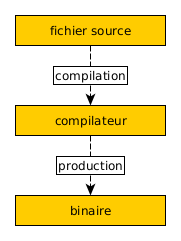
\includegraphics[scale=0.4]{../ressources/compilation.png}
            \caption{Fonctionnement de base d'un compilateur}
            \label{fig:compilateur}
          \end{figure}
        \end{center}
      \end{column}
      \begin{column}{.5\textwidth}
        \begin{figure}
          \centering
          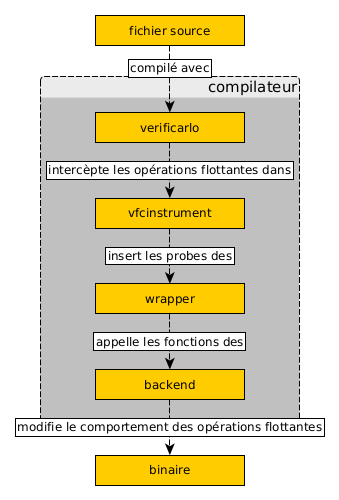
\includegraphics[scale=0.3]{../ressources/verificarlo_works.png}
          \caption{Fonctionnement de verificarlo}
          \label{fig:fonctionnement_verificarlo}
        \end{figure}
      \end{column}
    \end{columns}
  \end{block}
\end{frame}

\begin{frame}{Changements aux niveaux des backends}

  \begin{block}{Backend existant}
    ieee / vprec / mca / bitmask / cancellation / mca-mpfr
  \end{block}

  \begin{block}{Fonctions vectorielles en mode scalaire}
    \begin{itemize}
    \item mode par défaut
    \item tous les backends
    \end{itemize}
  \end{block}

  \begin{block}{Fonctions vectorielles en mode vectoriel}
    \begin{itemize}
    \item backend ieee
    \item backend vprec
    \end{itemize}
  \end{block}

\end{frame}

\begin{frame}{Changements aux niveaux du backend ieee}

  \begin{block}{Fonctionnement du backend}
    \begin{itemize}
    \item norme IEEE754
    \item fonction de débogue
    \end{itemize}
  \end{block}

  \begin{block}{Opérandes constantes}
    \begin{itemize}
    \item avertissement de clang sur les types des paramètres de fonction
    \item ajout d'un pragma pour retirer l'avertissement
    \end{itemize}
  \end{block}

\end{frame}

\begin{frame}{Changements aux niveaux du backend vprec}

  \begin{figure}
    \centering
    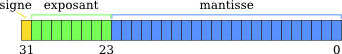
\includegraphics[width=200px]{../ressources/IEEE754_simple_precision.png}
    \caption{\label{fig:ieee_simple_precision}Représentation d'un nombre flottant simple précision}
  \end{figure}

  \begin{block}{Cas spéciaux}
    \begin{itemize}
    \item nombres infinis
    \item NaN (Not a Number - Pas un Nombre)
    \end{itemize}
  \end{block}

\end{frame}

\begin{frame}{Compilation}

  \begin{block}{Ajout à la compilation de Verificarlo}
    Compilation des \textbf{wrappers} et des \textbf{backends} avec le drapeau:
    \begin{center}
      \textbf{-march=native}
    \end{center}
  \end{block}

  \begin{block}{Avantage}
    Détection automatique des jeux d'instructions disponibles
  \end{block}


\end{frame}

\begin{frame}{Test}

  \begin{block}{Languages}
    \begin{itemize}
    \item bash (script de test)
    \item c (programme principale)
    \item python
    \end{itemize}
  \end{block}

  \begin{block}{Test}
    \begin{itemize}
    \item opérations arithmétiques vectorielles
    \end{itemize}
  \end{block}

\end{frame}


\begin{frame}{Test}

  \begin{block}{Bon résultat des opérations arithmétiques vectorielles}
    

  \centering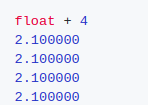
\includegraphics[scale=0.8]{../ressources/bon_resultat.png}

    
  \end{block}

  \begin{block}{Verification de l'appel aux probes vectorielles}
\centering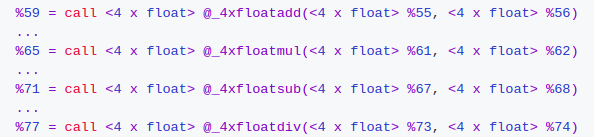
\includegraphics[scale=0.5]{../ressources/appel_des_fonction.png}
  \end{block}
\end{frame}

\begin{frame}{Test}

\begin{block}{Utilisation des jeux d'instructions vectoriels par le backend}
\centering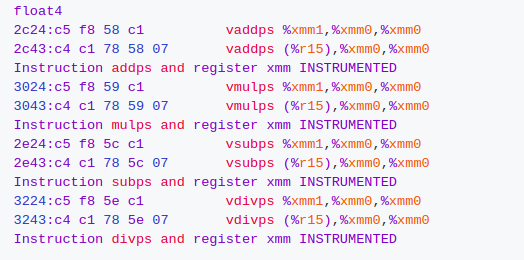
\includegraphics[scale=0.5]{../ressources/ajout_instructions.png}
  \end{block}
\end{frame}

\begin{frame}{Conclusion de la Vectorisation}

  \begin{block}{Fait}
    \begin{itemize}
    \item test opérations arithmétiques vectorielles simple
    \item probes vectorielles
    \item fonctions vectorielles (mode scalaire ou vectoriel)
    \item activation des jeux d'instruction
    \end{itemize}
  \end{block}

  \begin{alertblock}{Reste à faire}
    \begin{itemize}
    \item test des conditions vectorielles
    \item test des opérations vectorielles spécifique aux backends
    \item vectoriser les backends manquants
    \item test des performances
    \end{itemize}
  \end{alertblock}

\end{frame}

\begin{frame}{Conclusion}
 \begin{block}{Domaine étudié}
    \begin{itemize}
    \item Parallélisation
    \item Vectorisation
    \end{itemize}
  \end{block}
  
  \begin{block}{Cours en relation}
    Architecture Parallèle
  \end{block}

\end{frame}
 


\end{document}
